\section*{Code}

The code used to produce the plots is available at \url{https://github.com/hermanbrunborg/FYS4150-Project-3}

\subsection*{Appendix \romannumeral 1}
\label{analytical}

To test our implementation, we want to find a specific analytical solution given some initial conditions, and compare this with what our numerical approach gives us. Let us therefore assume we have a single charges particle in our Penning trap, with
%
\begin{align*}
x(0) = x_0, \quad \dot x(0) = 0, &\quad y(0) = 0, \quad \dot y(0) = v_0, \\
z(0) = z_0, \text{ an}&\text{d} \quad \dot z(0) = 0.
\end{align*}
%
Next, we use our general analytical solution for the $xy$-plane (eq \ref{eq:analytical_solution_xy}) to find a specific solution given the initial conditions listed above. We then get two equations
%
\begin{align}
A_+ e^0 + A_- e^0 &= x_0 \\
-i \omega_+ A_+ e^0 -i \omega_- A_- e^0 &= v_0 i,
\end{align}
%
which we can write as the matrix equation
\begin{equation*}
\begin{pmatrix}
1 & 1 & x_0 \\
-i\omega_+ & -i \omega_- & v_0 i
\end{pmatrix}
\sim
\begin{pmatrix}
1 & 0 & \frac{v_0 + x_0 \omega_-}{\omega_- - \omega_+} \\
0 & 1 & -\frac{v_0 + x_0 \omega_+}{\omega_- - \omega_+}
\end{pmatrix}.
\end{equation*}
%
This means that our specific solution in the $xy$-plane has
%
\begin{equation*}
A_+ = \frac{v_0 + x_0 \omega_-}{\omega_- - \omega_+} \quad 
A_- = -\frac{v_0 + x_0 \omega_+}{\omega_- - \omega_+}.
\end{equation*}
%
We then find the general analytical solution for the $z$-axis by finding the characteristic equation of (\ref{eq:ode_z}), which is $r^2 + \omega_z^2$, implying $r = \pm \omega_z i$. An ODE of this type, with a characteristic equation with two imaginary roots, has the general form
%
\begin{equation*}
    z(t) = C_1 \sin t + C_2 \cos t.
\end{equation*}
%
With our initial conditions, this becomes
%
\begin{equation*}
    z(t) = z_0 \cos t.
\end{equation*}
%
We use the specific analytical solutions above to test that our numerical implementations work properly.


\subsection*{Appendix \romannumeral 2}

\begin{figure}[H]
    \centering
    \text{Phase plot for two particles for x}
    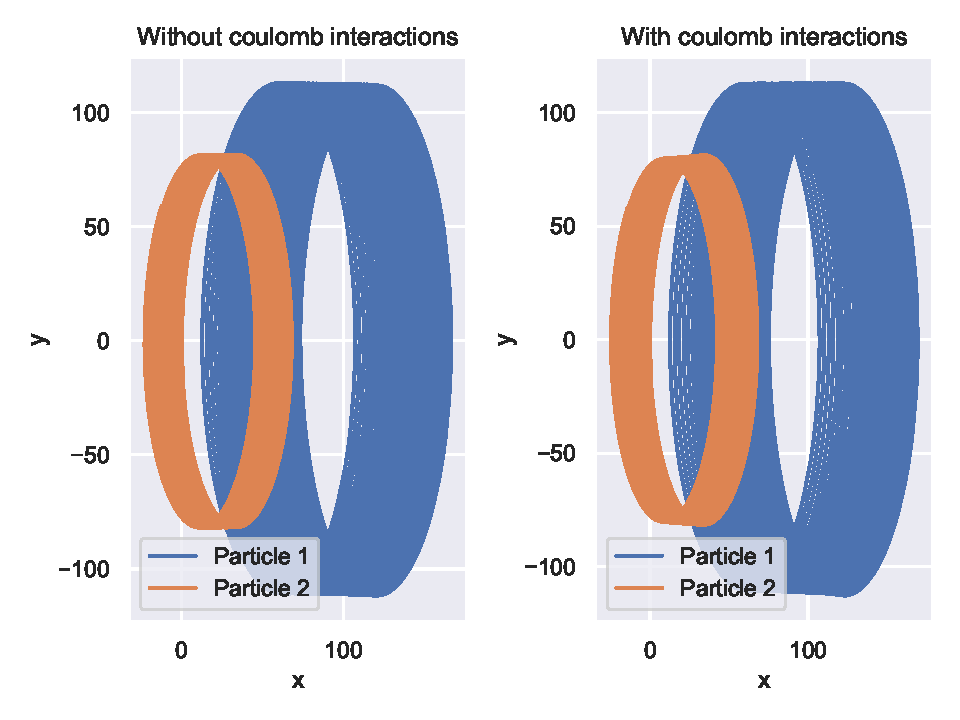
\includegraphics[width=0.5\textwidth]{data/phase_plots_two_particles_x.pdf}
    \caption{The phase plot for the particles in x-direction}
    \label{fig:phase_two_particles_x}
\end{figure}
\begin{figure}[H]
    \centering
    \text{Phase plot for two particles for y}
    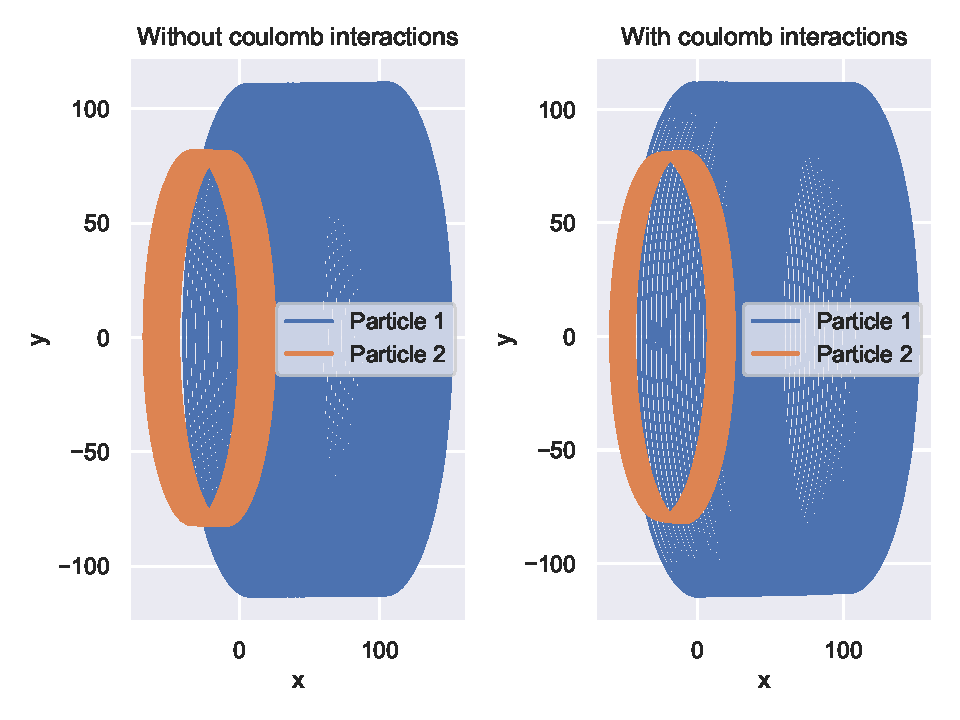
\includegraphics[width=0.5\textwidth]{data/phase_plots_two_particles_y.pdf}
    \caption{The phase plot for the particles in x-direction}
    \label{fig:phase_two_particles_y}
\end{figure}
\begin{figure}[H]
    \centering
    \text{Phase plot for two particles for z}
    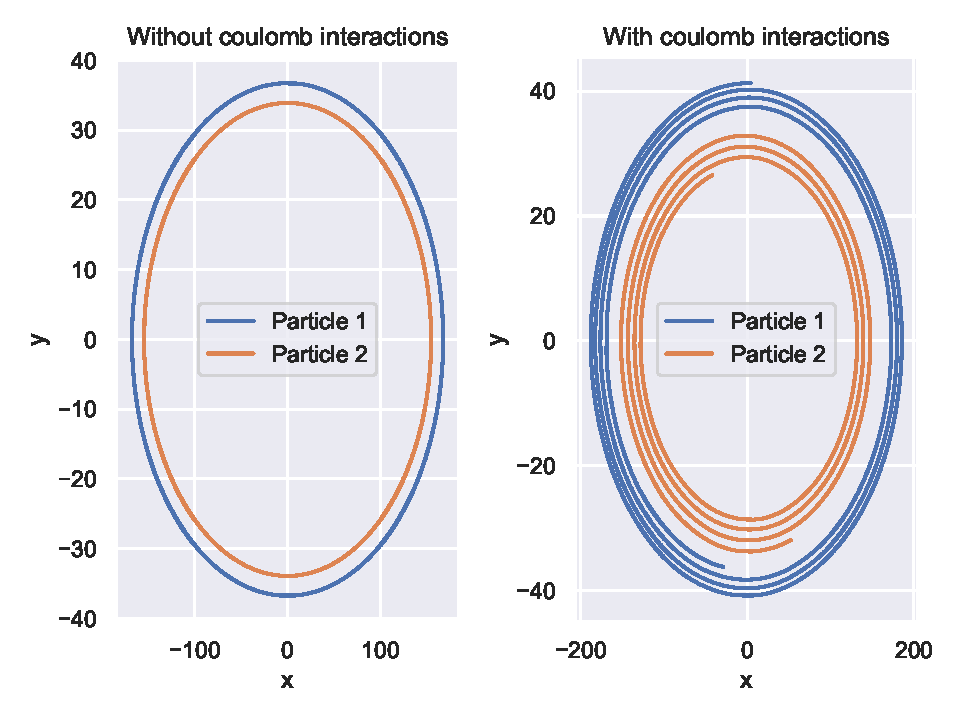
\includegraphics[width=0.5\textwidth]{data/phase_plots_two_particles_z.pdf}
    \caption{The phase plot for the particles in x-direction}
    \label{fig:phase_two_particles_z}
\end{figure}
